\subsection{Optimized emission output}
\label{sec:eval:maxout}

Given the insights from section~\ref{sec:eval:pumpspot}
we try to optimize the emitted output further.
The following
two optimization strategies
for the VECSEL output power
are proposed
based on a microscopic many-body physics simulation
\cite{Hader2011}.
The first is to AR coat the sample:
with a $3/4$-$\lambda$ coating
appropriate for the pump wavelength
the reflection from
the air--VECSEL cap interface
(in our case InP)
should reduce
without changing the conditions
for the emission wavelength.
This intervention
permits more of the incident pump
to enter the structure,
which increases the over all
wallplug efficiency.
The second optimization is
to use a reflecting metalization layer
behind the DBR --
while leaving the DBR transparent for the pump.
This results in
the pump light
passing the active region
once more.

We investigate these two strategies
in the lens configuration
with the achromatic lens
and a $333\,\mu\mathrm{m}$
pump spot diameter.
First,
we want to record the characteristics
of sample 1 in more detail.
Once we know these,
we can apply the AR coating
on this sample
in order to compare
with its uncoated state
directly.
For the second strategy
we have to use a different sample; sample 2.
Its specifications for the active region
and DBR are identical
with the ones from sample 1.
The difference
is a different treatment
of the gold layer
contacting the diamond heat sink:
by reducing the amount of Ti
used to adhere
the DBR to the gold,
this layer shows an increase
in reflectivity.

The light-light characteristics
resulting from this more detailed analysis
is shown in Fig.~\ref{img:LL_sample}.
Each data point
is measured $N=5$ times,
as opposed to only $N=3$
for section~\ref{sec:eval:pumpspot}.
The irradiated spot is labeled B
in Fig.~\ref{img:sample_surface}.
For this spot the sample
performed best.
On the other hand,
our setup is not designed
to scan the surface in a structured manner.
The found maximum could
be only a local maximum.

\begin{figure}
\centering
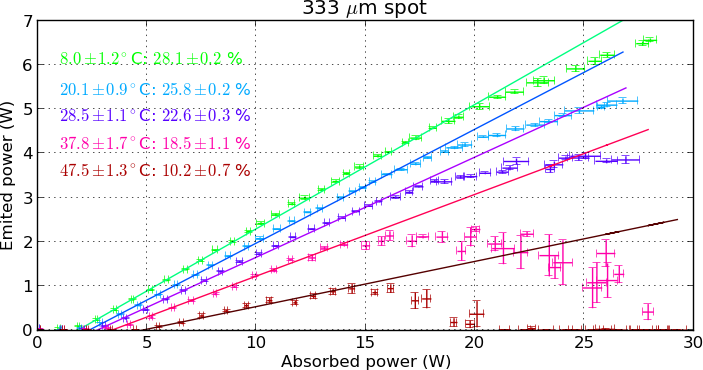
\includegraphics[width=14.5cm]{img/LL_sample.png}
\caption{Detailed LL of sample 1.
Irradiating spot B denoted in
Fig.~\ref{img:sample_surface}.
Each data point is measured $N=5$ times.
The error bars correspond
to the standard error.}
\label{img:LL_sample}
\end{figure}


\subsubsection{AR coating}
\label{sec:eval:maxout:AR}

The first optimization strategy
\cite{Hader2011}
is to apply
an anti-reflectance (AR) coating
on the sample.
In order to have
a direct comparison
we decided
to coat sample 1. 
However,
after this treatment,
the surface roughness
had visibly worsened.
In particular,
during aligning the output coupler,
in a first step we overlap
the pump spot with its reflection
from the output coupler,
using the visible aid
of a camera
along the emission path,
see appendix~\ref{app:alignment}.
Once we have found a lasing configuration
we rely on the power meter
to find the optimum alignment.

In the case of
the AR coated sample
the second spot
was hardly visible,
and looked patterned;
similar to a plastered wall.
Unsurprisingly,
the resulting light-light performance
is clearly weaker
than without the coating.
Figure~\ref{img:LL_sampleAR}
shows the resulted
light-light conversion.

Based on the stated observations,
we cannot compare
the two measurements.
We have to improve the coating process
before we can evaluate this optimization strategy.

\begin{figure}
\centering
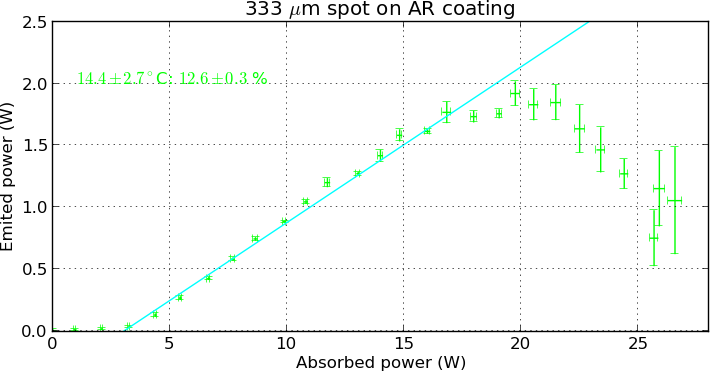
\includegraphics[width=14.5cm]{img/LL_sampleAR.png}
\caption{The AR coating
applied on sample 1 worsened its performance.
Given the observations made
during measurements
(see text),
this is a verdict most likely
not tenable for AR coating in general,
but concerns the quality of our coating in particular.}
\label{img:LL_sampleAR}
\end{figure}

\subsubsection{Reflecting metalization layer: record output}

For the second optimization strategy
\cite{Hader2011}
we use a sample
whose metalization interface
between DBR and CVD diamond
was treated to be highly reflective.
Sample 2 is measured
irradiating the spot
indicated with a red circle
in Fig.~\ref{img:sampled6_surface}.
The light-light characteristic
is depicted in Fig.~\ref{img:LL_sampled6}.

Apparently,
a lot more of the absorbed light
is converted into laser output
(nearly $60\,\%$
at \degr{5} heat sink temperature).
On the other hand,
the over all reflectivity off the sample
is higher for sample 2
than for sample 1.
This fact I revisit
in section~\ref{sec:eval:refl}. 

Table~\ref{tab:LL_sampled6} highlights
the observed peak performances.
These, coincidentally,
represent the new
(unofficial)
world record
in emitted power
in the $1300\,\mathrm{nm}$ waveband.
The highest reported emission power
for this waveband so far
was $7.1\,\mathrm{W}$
in a intracavity heat spreader configuration
using a pump spot diameter of $300\,\mu\mathrm{m}$
at a heat sink temperature
of \degr{7}
\cite{Sirbu2014OptExp}.

Figure~\ref{img:conversion_temp}
shows a comparison between
sample 1 (uncoated)
and sample 2.
The latter appears to be
about twice as efficient
in converting the absorbed light.
However,
this cannot directly be attributed
to the second pass
through the active region
with this optimized design.
In sample 1
we don't distinguish
whether the pump is absorbed
in the active or the metalization layer.
Our definition of absorbed power,
$A=P-R$ (\ref{eq:abspwr}),
looks only at the difference
of power in the pump
and the reflection channel.
The contribution
from the reflected power
is indeed larger
for sample 2,
discussed in section~\ref{sec:eval:refl}.

\begin{figure}
\centering
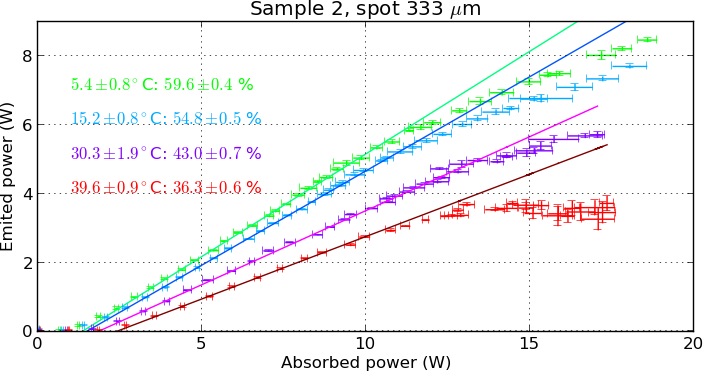
\includegraphics[width=14.5cm]{img/LL_sampled6.png}
\caption{Light light performance
of sample 2,
with the gold interface
between DBR and CVD diamond
treated to be highly reflective.
The irradiated spot
is indicated
in Fig.~\ref{img:sampled6_surface}.
Each data point
represents an average
over 5 repetitions.}
\label{img:LL_sampled6}
\end{figure}

\begin{table}[h]
\centering
\caption{Highlighting the peak data from Fig.~\ref{img:LL_sampled6}.
The error values correspond:
to the standard deviation for the heat sink,
and to the standard error (\ref{eq:sterr})
for the absorbed and emitted power.
Pump spot diameter is estimated
as $333\,\mu\mathrm{m}$.
The incidence angle
is $\approx36^\circ$.}
\begin{tabular}{rrr}
\hline
Heat sink (\degr{}) &
absorbed power ($\mathrm{W}$) & emitted power ($\mathrm{W}$) \\
\hline
$5.4\pm0.8$ & $18.6\pm0.3$ & $8.46\pm0.06$ \\
$15.2\pm0.8$ & $18.1\pm0.5$ & $7.7\pm0.06$ \\
$30.3\pm1.9$ & $17.1\pm0.2$ & $5.72\pm0.09$ \\
$39.6\pm0.9$ & $17.4\pm0.2$ & $3.7\pm0.2$ \\
\hline
\end{tabular}
\label{tab:LL_sampled6}
\end{table}

\begin{figure}
\centering
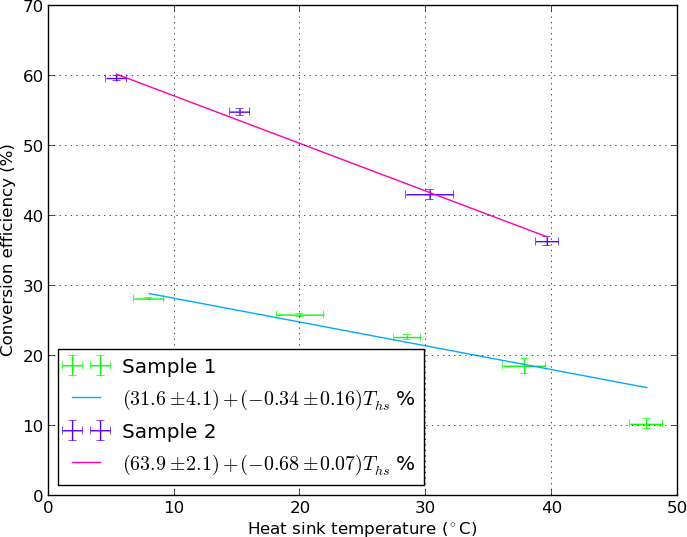
\includegraphics[width=14.5cm]{img/conversion_temp.png}
\caption{Summary of the values found in
Fig.~\ref{img:LL_sample} and \ref{img:LL_sampled6}.
The conversion efficiency of sample 2
corresponds to approximately twice
the value of sample 1.
The ultimate limit of conversion efficiency
is given by the quantum defect
$\lambda_\mathrm{pump}/\lambda_\mathrm{laser}=77.5\,\%.$}
\label{img:conversion_temp}
\end{figure}